% ============================================================
%  GamefyDB — PFE Report  |  Chapters 1 & 2
%  Author: Sarra Mediouni
%  Compile with pdflatex (or XeLaTeX for UTF-8 support).
% ============================================================

\documentclass[12pt, a4paper]{report}

% ---------- packages ----------
\usepackage[T1]{fontenc}
\usepackage[utf8]{inputenc}
\usepackage[english]{babel}
\usepackage{geometry}
\usepackage{graphicx}
\usepackage{hyperref}
\usepackage{booktabs}
\usepackage{array}
\usepackage{longtable}
\usepackage{enumitem}
\usepackage{titlesec}
\usepackage{fancyhdr}
\usepackage{xcolor}
\usepackage{listings}
\usepackage{caption}
\usepackage{subcaption}
\usepackage{float}
\usepackage{microtype}

\geometry{top=2.5cm, bottom=2.5cm, left=3cm, right=2.5cm}

% ---------- placeholder for figures still to be captured ----------
\newcommand{\todoFigure}[2][0.7\textwidth]{%
  \fcolorbox{red!60!black}{red!5}{%
    \parbox{#1}{\centering\vspace{0.6cm}%
      \textcolor{red!60!black}{\textbf{[TODO --- insert figure]}}\\[4pt]
      \textit{#2}\vspace{0.6cm}}}%
}

% ---------- header / footer ----------
\pagestyle{fancy}
\fancyhf{}
\fancyhead[L]{\small GamefyDB}
\fancyhead[R]{\small \leftmark}
\fancyfoot[C]{\thepage}
\renewcommand{\headrulewidth}{0.4pt}

% ---------- chapter title style ----------
\titleformat{\chapter}[display]
  {\normalfont\Large\bfseries\color{black}}
  {\chaptertitlename\ \thechapter}{10pt}{\Huge}
\titlespacing*{\chapter}{0pt}{-10pt}{20pt}

% ============================================================
\begin{document}

% ============================================================
%  CHAPTER 1 — GENERAL CONTEXT OF THE PROJECT
% ============================================================
\chapter{General Context of the Project}

\section{Introduction}

This opening chapter sets the scene for the internship work that
follows. It first introduces the company that hosted the project, then
walks through how the centre currently operates, points out where the
existing setup falls short, and lays out the solution put forward to turn
the raw operational data into something the manager can actually rely on
day to day. The chapter closes on the project-management framework retained
for the four months of work.

\section{Host Organisation Presentation}

\textbf{Gamefy Academy} sits in \textbf{La Soukra}, on the northern
edge of Tunis, and opened its doors in 2025. The clientele leans young
and the atmosphere is sociable --- people come to play together rather
than to grind alone at home. Three things bring them in: a row of
high-end PC stations, two PlayStation~5 setups (one of them tucked
into a private VIP booth), and a small snack bar that sells drinks
(water, soda, Schweppes, Redbull) and cookies to go with a long
session. The wider context helps: gaming has been gaining ground
visibly in Tunisia over the past few years, and a loyalty programme
backed by a small set of named accounts in the point-of-sale software
gives the centre a stable base of returning members.

\begin{figure}[H]
  \centering
  \todoFigure[0.4\textwidth]{Insert the official Gamefy Academy logo here
  (transparent-background PNG provided by the owner).}
  \caption{Gamefy Academy's logo.}
  \label{fig:gamefy_logo}
\end{figure}

\subsection{Organisational Structure of Gamefy Academy}

Operations at Gamefy Academy rest on a compact team and a small set of clearly
identified accounts within the point-of-sale software. The owner manages the
establishment and supervises the staff. Five named cashier accounts, namely
\textit{taktek}, \textit{yassine}, \textit{youssef}, \textit{monta}, and
\textit{guds}, handle the customer-facing activity. A shared
\textit{cashier} profile is used during shift hand-offs, and a dedicated
\textit{admin} account is reserved for the owner. Each cashier supervises one
or more terminals during a shift, opens and closes gaming sessions, rings up
snack-bar purchases, and processes top-ups for the loyalty members. The
following organisational chart illustrates this structure.

\begin{figure}[H]
  \centering
  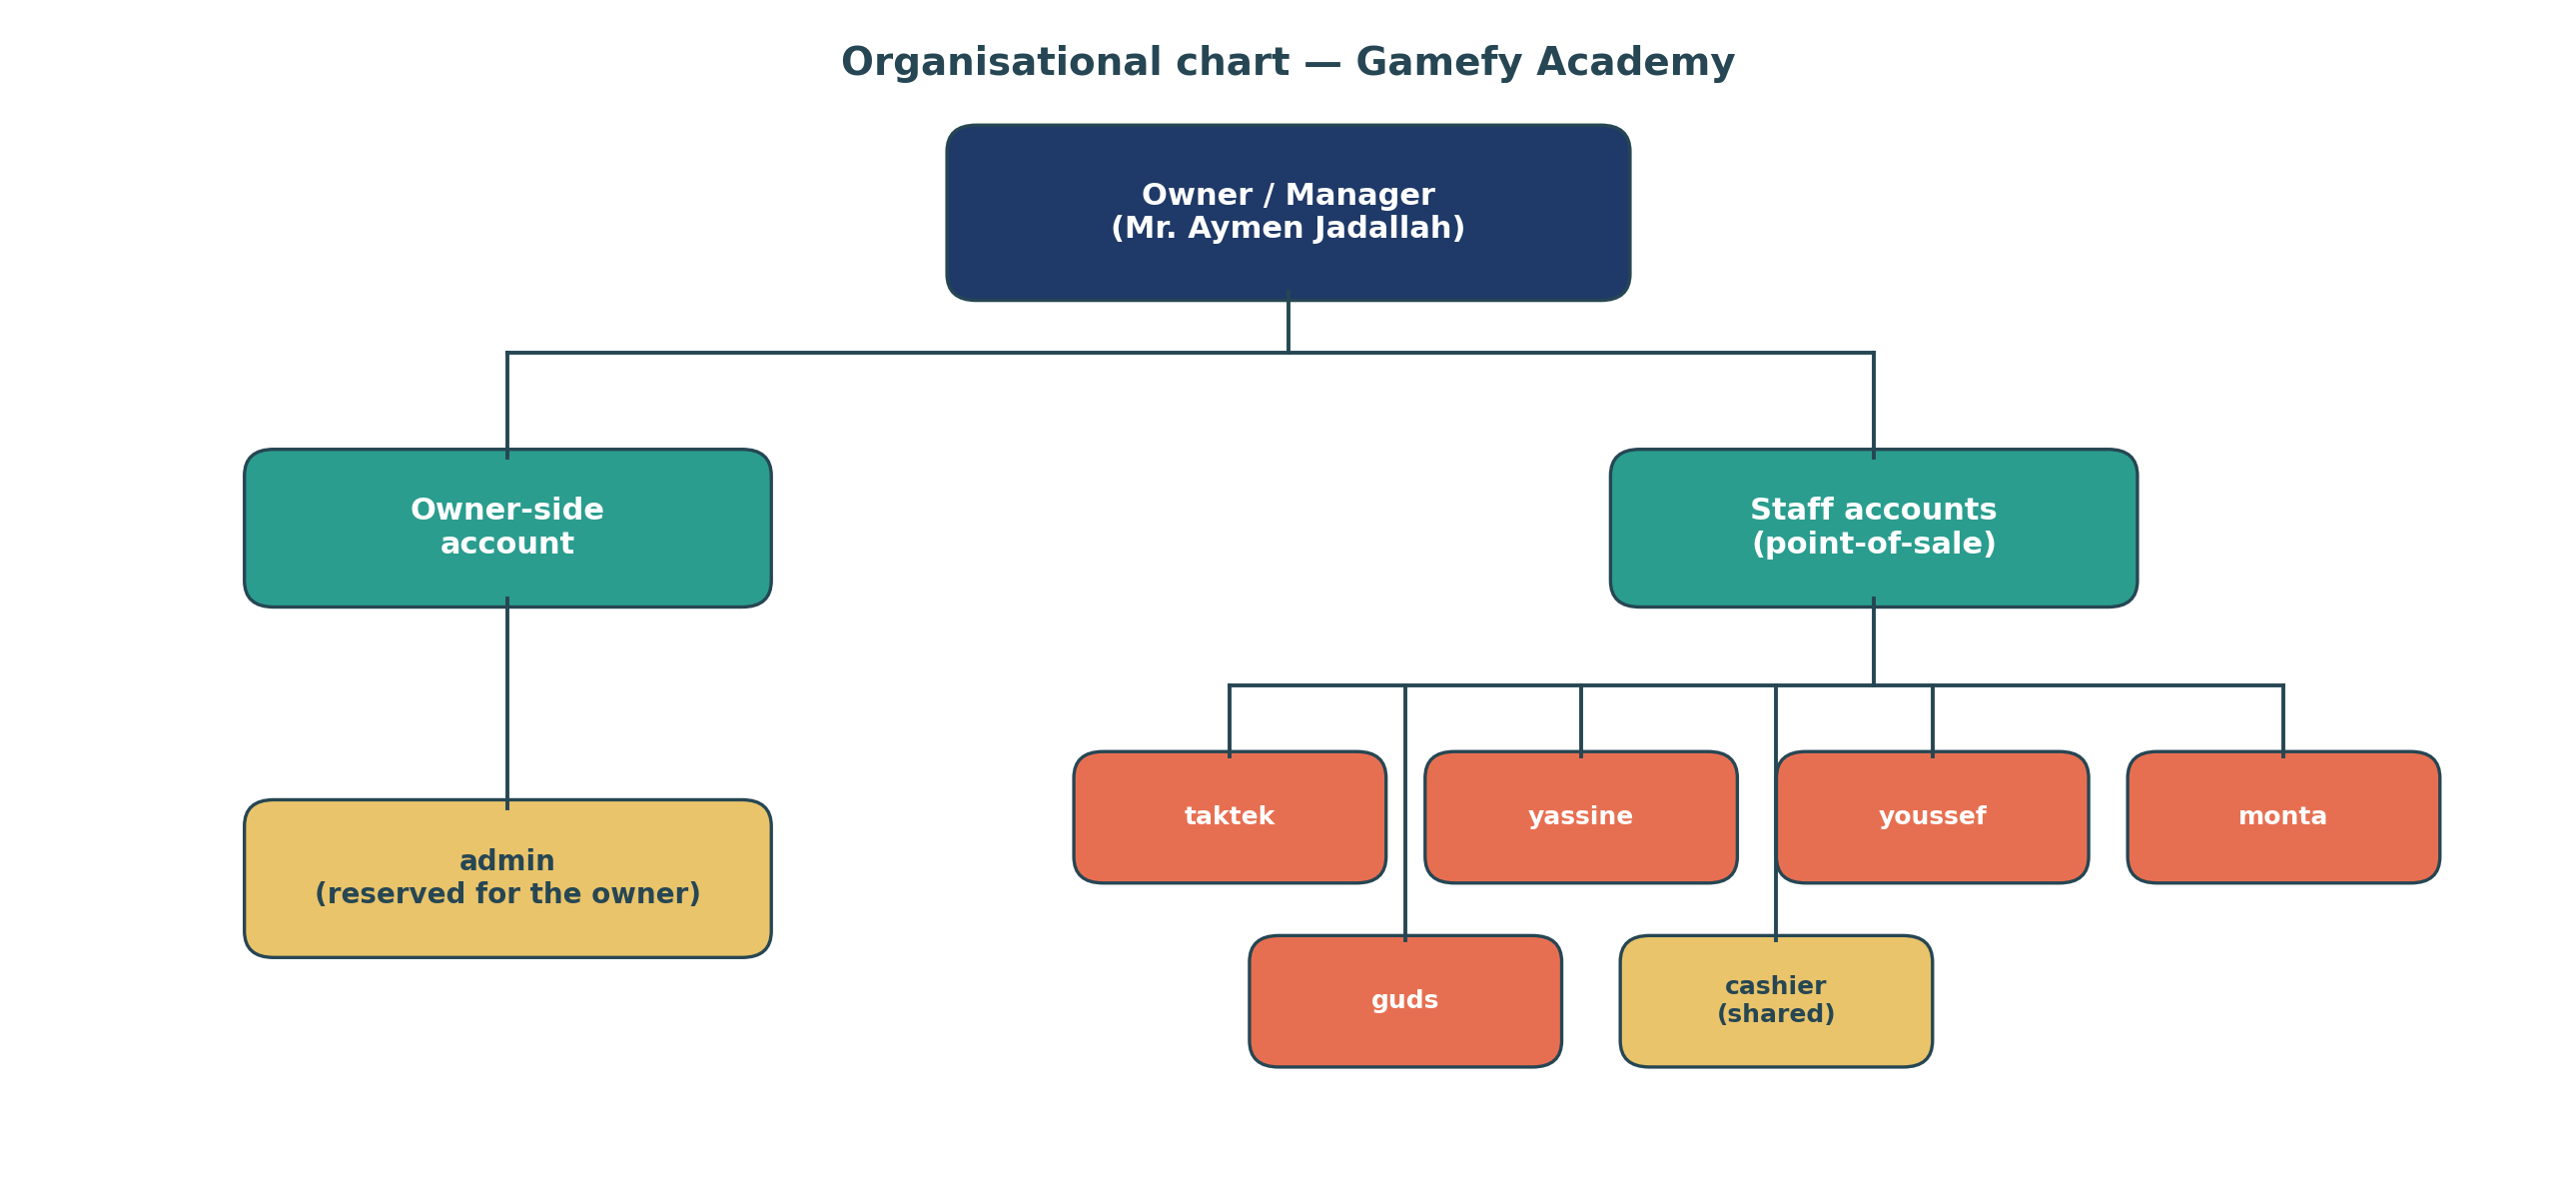
\includegraphics[width=0.85\textwidth]{images/org_chart.png}
  \caption{Organisational chart of Gamefy Academy.}
  \label{fig:org_chart}
\end{figure}

\subsection{Services provided by the company}

Gamefy Academy provides a portfolio of services oriented around three
activity areas. Gaming on terminals is the core activity. Sixteen active
terminals are made available to the customers, including ten standard PC
workstations (\textsc{GAMEFY01} to \textsc{GAMEFY10}), two PlayStation~5
consoles (\textsc{PS5\,(1)} and \textsc{PS5\,(2)}), and a private VIP booth
(\textsc{GAMEFY-VIP}). Three additional \textsc{DESKTOP} machines are used
internally by the staff for back-office tasks. The snack bar accompanies the
gaming activity and supplies drinks and cookies; alongside it, the same
point-of-sale system also handles a small line of accessory items
(USB keys, headset replacements and the like) sold at the counter. A
loyalty programme rewards regular customers with reduced rates and tracks
their cumulative time on the terminals as well as their cumulative spend.

\section{Project Presentation}

This section introduces the project in a structured way. It first sets the
academic context, then analyses the current situation, identifies the
weaknesses of the existing arrangement, formulates the problem to be addressed,
and concludes with the solution put forward in response.

\subsection{General context of the project}

The work presented here was carried out as part of a Bachelor's
Business Computing degree, BI specialisation, delivered
by ISIMA --- the computer-science institute in Mahdia attached to the
University of Monastir. The accompanying four-month internship took
place at Gamefy Academy, under joint supervision from an ISIMA mentor
and the owner of the centre. The brief was to build a complete,
data-driven solution covering both descriptive and predictive uses of
the centre's operational data, through three connected pieces:
dashboards, machine-learning models and a conversational interface.

\subsection{Analysis of the Existing System}

At the time the internship started, the centre relied on a single
information flow. The point-of-sale software was capable of exporting four
\texttt{.xls} reports on demand, covering the cash transactions, the gaming
sessions, the stock movements, and the loyalty members. The exports were
saved into a local folder on the owner's machine. Beyond this storage step,
no further processing took place. No pipeline cleaned the files, no
dashboard consumed them, and no analytical model fed back into the
decision-making process. Whenever the owner needed an answer to a business
question, such as which cashier had had the best month, which terminal was
the most popular, or whether revenue was trending upwards, the only available
option was to open the corresponding spreadsheet and to assemble a pivot
table by hand. In practice this rarely happened, and most of the data
accumulated without ever being analysed.

\subsection{Criticism of the Current System}

A close examination of the current arrangement is a necessary step before
proposing any improvement, since it allows the limitations of the existing
workflow to be made explicit and the areas of greatest impact to be
identified. The review performed during the early phase of the internship
revealed several weaknesses in the way the operational data is currently
exploited at the centre:

\begin{itemize}
  \item \textbf{Absence of an automated pipeline:} the four Excel exports
        are produced on demand and stored locally, but no software exists
        that would transform them into a clean analytical dataset. As a
        result, every analysis requires a manual intervention on the raw
        files.
  \item \textbf{Manual decision-support:} pivot tables built ad hoc inside
        Excel are the only available reporting medium. Such tables are
        time-consuming to assemble, prone to copy-and-paste errors, and
        rarely updated, which limits the responsiveness of the manager.
  \item \textbf{Hidden data-quality artefacts:} the exports contain a
        number of structural irregularities that remain invisible when a
        spreadsheet is opened in Excel but that severely complicate any
        automated processing. These include page-break artefacts,
        non-standard number formats, merged-cell column shifts, missing
        cashier names, inconsistent totals, and footer rows.
  \item \textbf{Lack of forward-looking analysis:} no model has ever been
        applied to the data, so the centre cannot anticipate revenue
        evolution, detect abnormal days, or estimate the future activity of
        its loyalty members.
  \item \textbf{Limited accessibility of information:} the data is locked
        inside Excel files that only the owner consults. There is no
        unified interface through which the manager could obtain a
        synthetic view of the centre's activity, let alone interact with
        the data in plain language.
\end{itemize}

In summary, Gamefy Academy collects detailed operational data continuously,
but the absence of an automated pipeline, the manual nature of the
reporting, and the lack of any analytical layer prevent that data from
being turned into a useful decision-support resource. The point-of-sale
exports themselves carry several structural irregularities that worsen the
situation by making automated processing harder than it should be. The
detail of these artefacts is summarised in Table~\ref{tab:dq}.

\begin{table}[H]
  \centering
  \caption{Data-quality issues observed in the source files.\label{tab:dq}}
  \begin{tabular}{p{3.5cm} p{9.5cm}}
    \toprule
    \textbf{Issue} & \textbf{Description} \\
    \midrule
    Page-break artefacts
      & The exporter inserts a \textit{Page~X/Y} row, two empty rows, and a
        copy of the header line roughly every forty data rows. \\[4pt]
    Non-standard number format
      & TND amounts use a narrow no-break space
        (\texttt{\textbackslash u202f} or \texttt{\textbackslash xa0}) as a
        thousands separator and a comma as a decimal mark. Common parsers
        reject both conventions. \\[4pt]
    Merged-cell column shift
      & Merged cells in the visible layout shift the actual data column
        index relative to the header, which makes automatic header
        detection unreliable. \\[4pt]
    Missing cashier names
      & Sub-total rows inserted between blocks of data carry a generic
        label in the cashier column rather than the corresponding account
        name. \\[4pt]
    Inconsistent totals
      & Several session and stock rows show recorded totals that do not
        match the sum of their components, suggesting either rounding or
        data-entry errors in the source software. \\[4pt]
    Footer rows
      & The members file ends with a \textit{Report Result\,:} footer
        whose numeric totals occupy what otherwise looks like a data row. \\
    \bottomrule
  \end{tabular}
\end{table}

\subsection{Problematic}

Gamefy Academy generates a continuous stream of operational data through its
point-of-sale software, yet very little of that data is currently turned
into actionable insight. The exports are usable in their raw form only by an
analyst familiar with the structural irregularities they contain, and even
then the resulting analyses are slow, manual, and reserved to exceptional
situations. The absence of an automated pipeline, of a dashboarding layer,
and of any predictive component prevents the centre from monitoring its
performance in real time, anticipating future activity, and detecting
abnormal events. The central question addressed in this work can therefore
be formulated as follows: \textit{how can the raw, artefact-laden Excel
exports produced by the point-of-sale system be transformed in a reliable
and repeatable manner into a clean analytical dataset, and exploited to
support both descriptive and predictive decision-making at the centre?}

\subsection{Proposed Solution}

To address the limitations identified above, this project proposes
\textbf{GamefyDB}, an end-to-end Business Intelligence solution dedicated to
the operational data of Gamefy Academy. The objective of the proposal is to
provide the owner with an automated, repeatable, and complete data flow that
covers everything from the cleaning of the raw exports to the natural-language
interrogation of the resulting dataset. The solution is articulated around
five complementary components:

\begin{itemize}
  \item \textbf{ETL Pipeline:} a Python module
        (\texttt{gamefydb/pipeline.py}) that reads the four source files,
        strips the page-break artefacts, parses the non-standard number and
        date formats, restores the missing cashier names, and assembles a
        six-table star schema composed of four dimensions and two fact
        tables, all executable from a single command.
  \item \textbf{Power~BI Dashboards:} an interactive
        Power~BI report (\texttt{gamefyyy.pbix}) organised around four
        pages, namely revenue overview, rankings, live operations, and shift
        reporting, with all the relationships and DAX measures required to
        support the agreed KPIs.
  \item \textbf{Forecasting Module:} five forecasting routines covering
        revenue, member activity, peak hours and days, session volume, and
        stock replenishment, with an internal comparison between Prophet,
        SARIMA, and XGBoost on an 80/20 chronological split, including the
        possibility of an Open-Meteo weather regressor on Prophet and
        XGBoost.
  \item \textbf{Segmentation and Anomaly Detection:} a K-Means clustering
        that splits the loyalty members into four behavioural profiles and
        produces a continuous loyalty score, together with a day-of-week
        Z-score detector that flags revenue, session-volume, and
        member-activity outliers with a mild or severe severity grading.
  \item \textbf{Conversational Assistant:} a Streamlit application
        (\texttt{app.py}) that lets the owner ask questions in English,
        French, or Arabic, by typing or by voice, and that returns both a
        written answer and a relevant chart.
\end{itemize}

Because the real exports cover less than a year of activity ---
not long enough for a model that needs to see at least one full
yearly cycle --- a sixth component is bolted onto the chain: a
synthetic data generator (\texttt{gamefydb/data\_generator.py}),
which extends the history backwards by sampling from the real
daily-revenue distribution and modulating it with Ramadan, Eid,
monthly and weather-driven multipliers. Together, these
components turn the raw exports into a continuously updated, analytical, and
conversational decision-support solution.

\section{Project Management Methodologies Study}

Project management plays a fundamental role in the execution of a Business
Intelligence project, since it determines how the work is organised, how the
progress is monitored, and how changes in requirements are absorbed during
the development. A project management methodology can be defined as a
structured set of practices and processes that guide the team through the
project lifecycle. Several methodologies coexist in the literature, each one
adapted to a specific class of projects. This section presents two such
methodologies, namely GIMSI and Scrum, and compares them on the criteria
that matter the most for the present work.

\subsection{The GIMSI Method}

The GIMSI methodology is a project management approach designed specifically
for decision-support and Business Intelligence projects. It was developed in
a French-speaking environment and covers the full lifecycle of a Business
Intelligence solution, from the identification of the business needs to the
operational deployment of the system.

\subsubsection{GIMSI objectives}

GIMSI pursues the following objectives:

\begin{itemize}[noitemsep]
  \item Organise the work of the project in a methodical and repeatable
        manner.
  \item Maintain a consistent alignment between the analysis of the needs,
        the design of the solution, and the final deliverable.
  \item Bring all the stakeholders together around a common decision-support
        objective.
  \item Capitalise on the knowledge produced during the project so that it
        can be reused in subsequent initiatives.
\end{itemize}

\subsubsection{Main Phases of GIMSI}

GIMSI runs through five sequential phases, shown in
Figure~\ref{fig:gimsi}:

\begin{enumerate}[noitemsep]
  \item \textbf{Preliminary Study:} justification of the project, study of
        the context, and identification of the decision-making needs.
  \item \textbf{Opportunity Study:} feasibility analysis and comparison of
        candidate solutions.
  \item \textbf{Detailed Study:} specification of the functional
        requirements and modelling of the target system.
  \item \textbf{Implementation:} development, integration, and deployment
        of the solution.
  \item \textbf{Permanent Improvement:} refinement of the system on the
        basis of operational feedback after go-live.
\end{enumerate}

\begin{figure}[H]
  \centering
  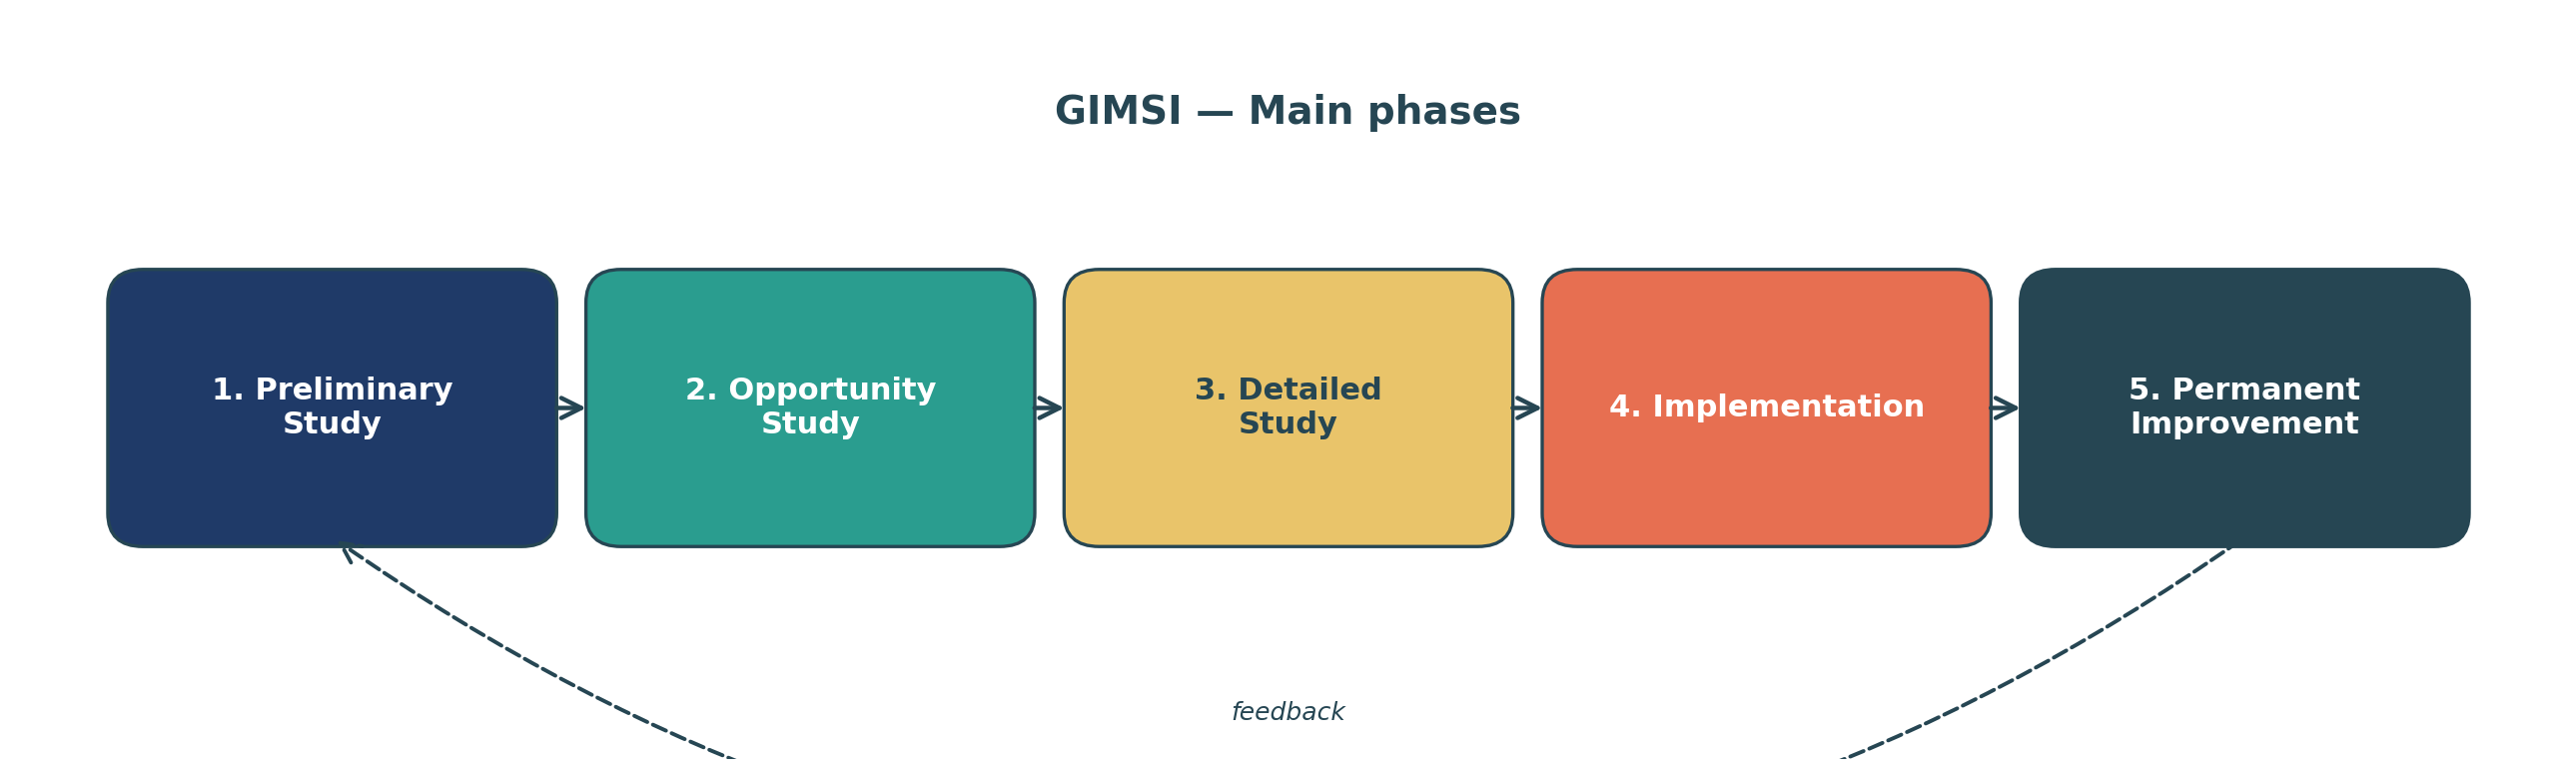
\includegraphics[width=0.75\textwidth]{images/gimsi.png}
  \caption{Main phases of GIMSI.}
  \label{fig:gimsi}
\end{figure}

\subsubsection{Advantages of GIMSI}

The GIMSI methodology offers several advantages, in particular:

\begin{itemize}[noitemsep]
  \item A complete documentation of the work at every phase, which improves
        the traceability of the design decisions.
  \item A well-structured framework that is well adapted to complex
        Business Intelligence projects.
  \item A global vision of the target system established from the very
        beginning of the project.
\end{itemize}

\subsection{SCRUM Methodology}

Scrum is an agile project management framework built around continuous
adaptation, close collaboration with the stakeholder, and the regular
delivery of working increments. It is particularly suited to projects whose
requirements are expected to evolve over time, which is typical of software
development. The Scrum process is illustrated in Figure~\ref{fig:scrum}.

\begin{figure}[H]
  \centering
  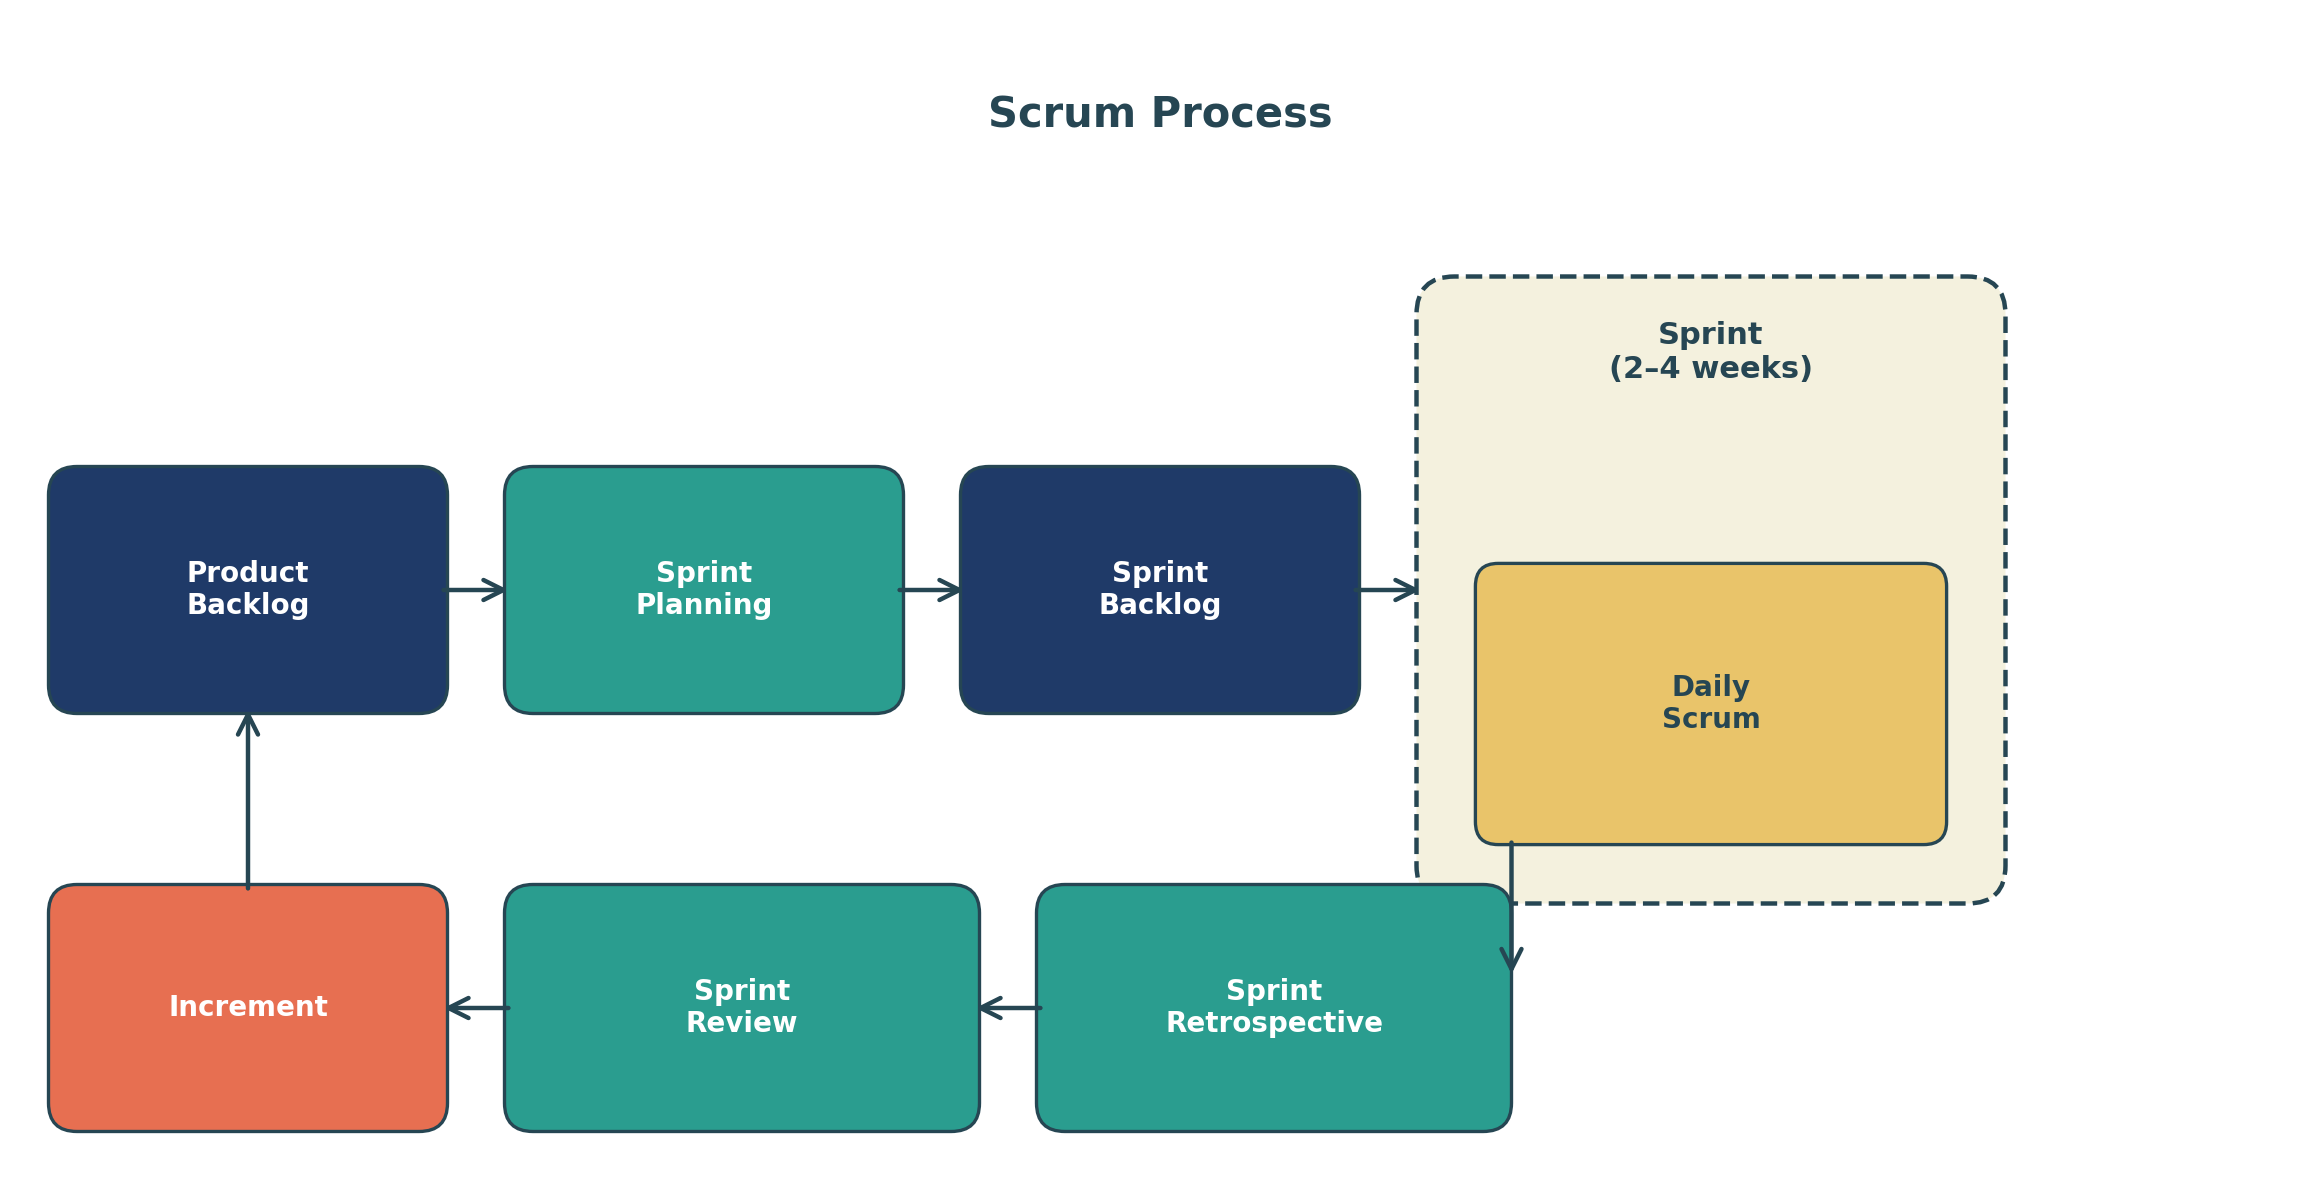
\includegraphics[width=0.75\textwidth]{images/scrum_process.png}
  \caption{Scrum process.}
  \label{fig:scrum}
\end{figure}

\subsubsection{Key Principles of Scrum}

Scrum rests on four core principles:

\begin{itemize}
  \item \textbf{Iterative and Incremental:} the work is broken into
        short cycles called sprints --- typically two to four weeks
        long --- and each sprint closes on a working increment of the
        product.
  \item \textbf{Well-Defined Roles:} Scrum is built around three
        complementary roles, illustrated in Figure~\ref{fig:scrum_roles}:
        \begin{itemize}
          \item \textit{Product Owner:} owns the product vision and
                orders the backlog by business value.
          \item \textit{Scrum Master:} owns the application of the
                Scrum framework, removes impediments, and supports the
                team in its daily work.
          \item \textit{Development Team:} self-organised and
                cross-functional, in charge of delivering the increment
                they committed to when the sprint started.
        \end{itemize}
  \item \textbf{Continuous Delivery:} a release-ready product increment
        is produced at the close of every sprint.
  \item \textbf{Scrum Ceremonies:} four recurring events frame the
        work of the team --- Sprint Planning, Daily Scrum, the review
        meeting at sprint end and the retrospective that follows it.
\end{itemize}

\begin{figure}[H]
  \centering
  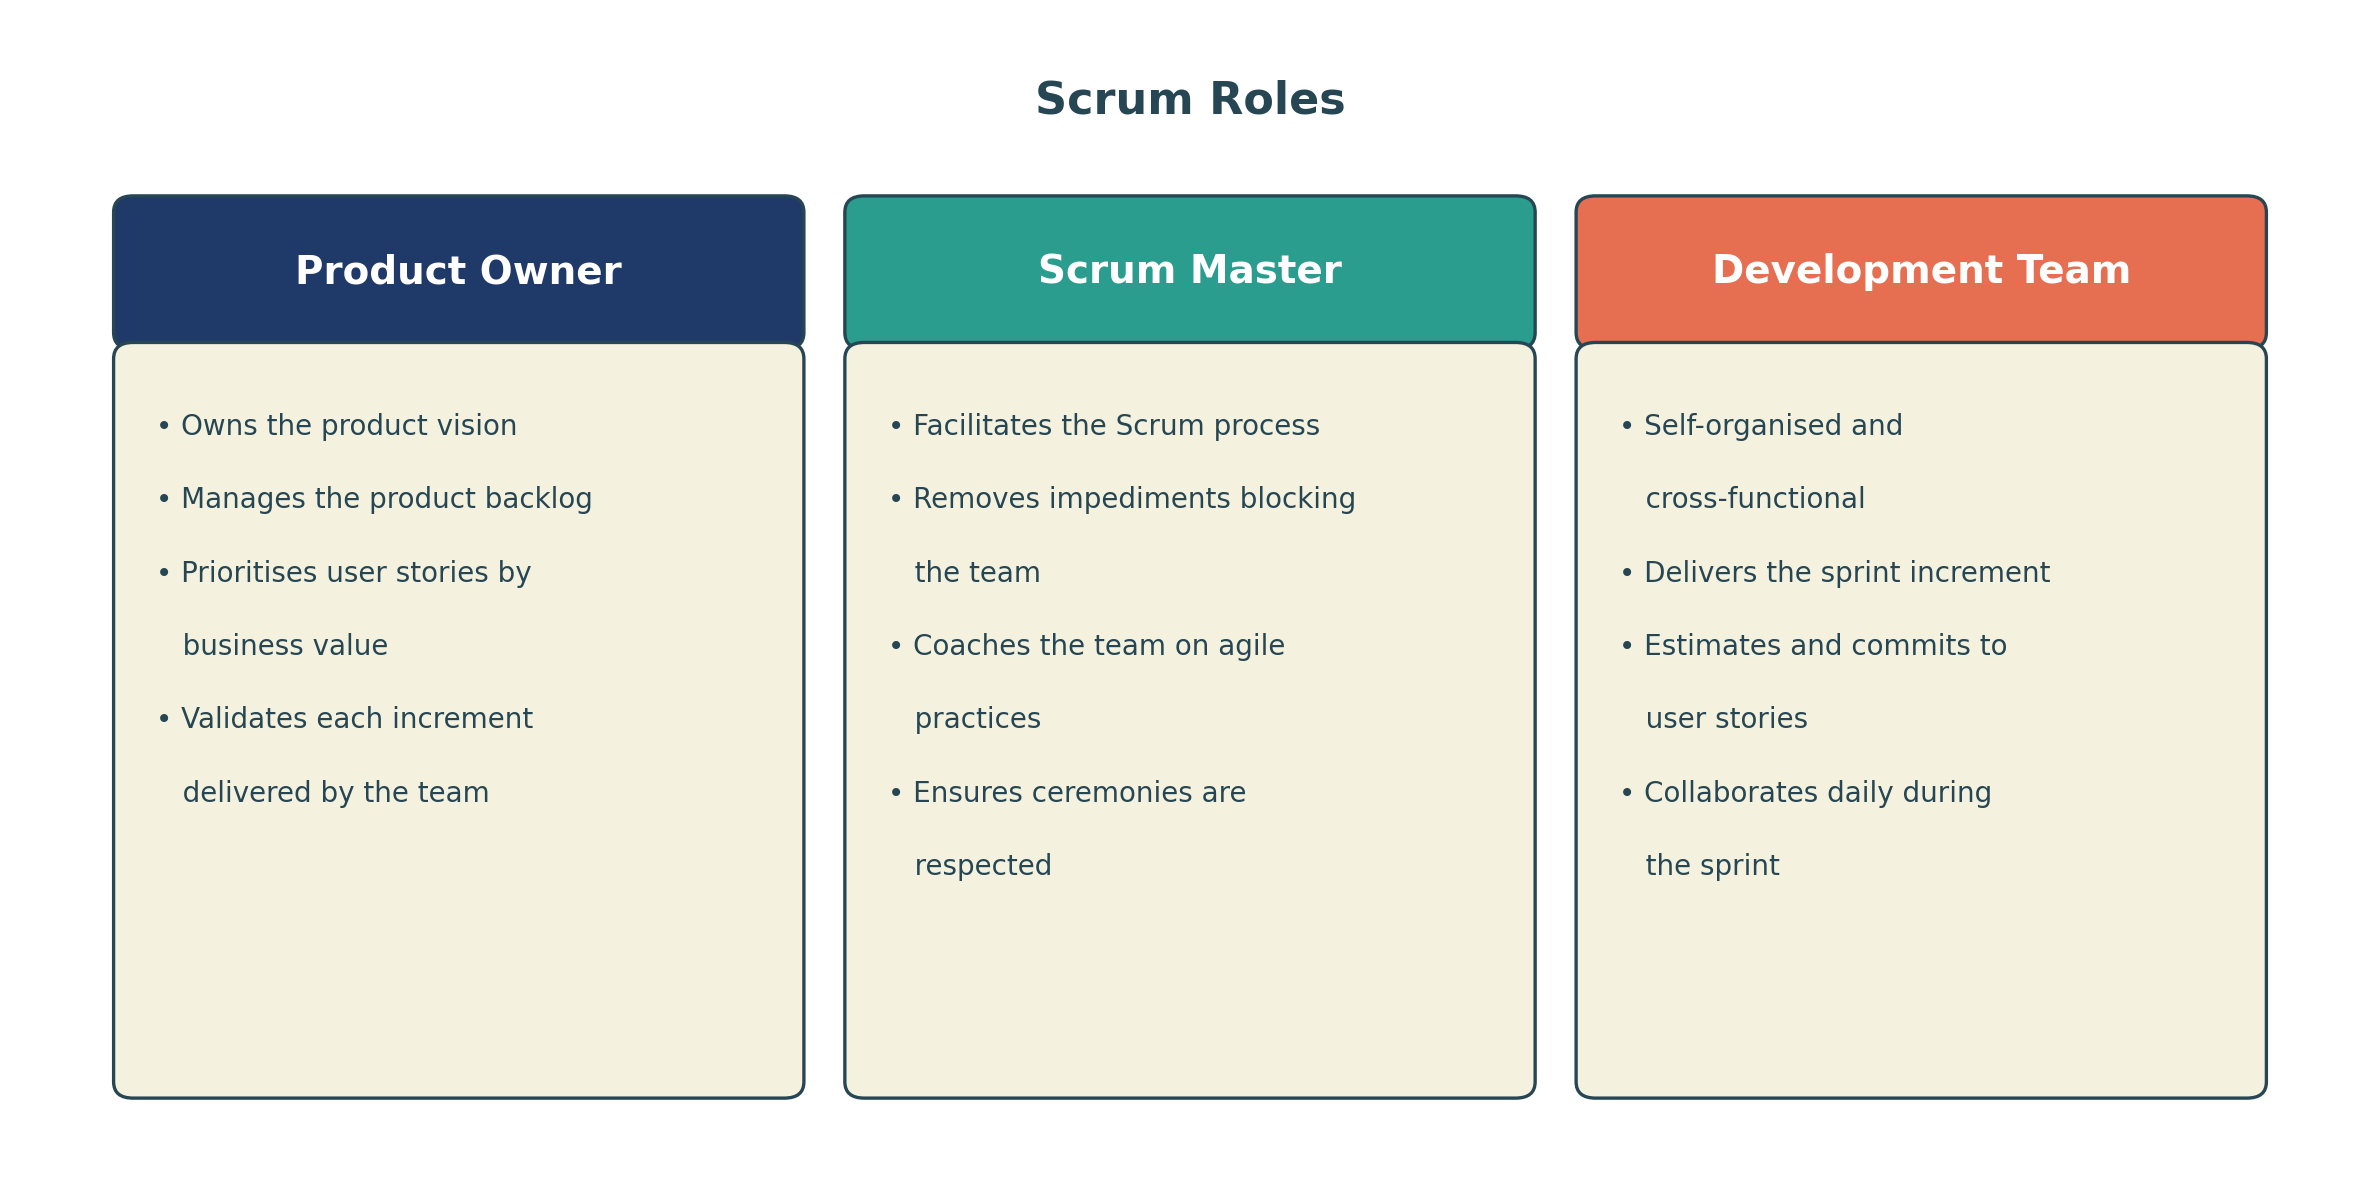
\includegraphics[width=0.75\textwidth]{images/scrum_roles.png}
  \caption{Scrum roles.}
  \label{fig:scrum_roles}
\end{figure}

\subsubsection{Advantages of Scrum}

Scrum offers a number of advantages that justify its use in projects where
the requirements are subject to change:

\begin{itemize}[noitemsep]
  \item A high responsiveness in the face of evolving requirements.
  \item A continuous engagement of the stakeholder throughout the project.
  \item A culture of continuous improvement supported by the
        retrospectives.
  \item A full visibility on the progress of the project at any point in
        time.
\end{itemize}

\subsection{Adopted Methodology}

Scrum is the framework retained for this work. The decision was
driven by the level of uncertainty around the source data at the
start of the internship. The data-quality issues described
earlier in this chapter were unknown when the work began, and any attempt to
specify the full system in advance would have led to assumptions that the
real files would later contradict. The iterative nature of Scrum allowed the
first sprint to be dedicated to the inspection and the cleaning of the
exports, and the dimensional model to be designed in the following sprint on
the basis of a verified dataset. The framework also accommodated the
addition of the machine-learning and the chatbot sprints, which were
introduced by the Product Owner once the cleaned data had become available
and the perimeter of what could realistically be built had been clarified.

\section{Conclusion}

So this is where the project starts: a small gaming centre in La Soukra
with under a year of \texttt{.xls} exports nobody had time to analyse,
and a clear gap between the data it collects every shift and the
decisions the owner actually makes from it. The shape of the answer
--- an ETL pipeline, a Power~BI report, an ML layer and a chatbot,
all driven from one command and wrapped in a Scrum cadence ---
follows naturally from that gap, but the details still have to be
filled in. Sprint~0, covered next, is where they are.

% ============================================================
%  CHAPTER 2 — SPRINT 0: PREPARATION PHASE
% ============================================================
\chapter{Sprint 0: Preparation Phase}

\section{Introduction}

Sprint~0 is the preparation sprint of the project. No deliverable ships at
its conclusion, but the entire success of the implementation work depends on
what is decided during this phase. The activities of Sprint~0 cover the
identification of the system actors, the elicitation of the functional and
non-functional constraints, the construction of the product backlog, the
choice of the technical architecture, and the design of the dimensional
model. This chapter describes each of these activities in turn.

\section{Requirements specification}

Pinning down requirements is among the most consequential stages of
a Business Intelligence project: it shapes every design decision
that comes after. When the specification is clear, the resulting
system tends to land where the business and the end-users actually
needed it to.

\subsection{Identification of system actors}

In UML terminology, an actor stands for any role --- human or
external system --- that exchanges something with the application,
whether to trigger a task or to consume one of its services.
Identifying actors comes before requirement modelling because it
fixes the responsibilities and access rights expected of each category
of user. Three actors interact with GamefyDB.

\begin{itemize}
  \item \textbf{The Gaming Centre Owner / Manager:} the principal
        stakeholder. The owner uses the Power~BI dashboards in his daily
        routine, reads the forecasts and the anomaly alerts when planning
        the weeks ahead, and questions the conversational assistant for
        quick clarifications during a shift.
  \item \textbf{The Data Analyst / BI Developer:} the role occupied by the
        author of the report throughout the internship. The analyst
        executes the pipeline, verifies the output, maintains the
        Power~BI report, and adds new machine-learning or chatbot features
        as the requirements evolve.
  \item \textbf{The Cashier:} an indirect actor. Cashiers do not interact
        with GamefyDB directly, but their daily activity recorded into the
        point-of-sale software is precisely what produces the four Excel
        exports on which the entire system depends.
\end{itemize}

\subsection{Functional requirements}

The functional requirements describe the features expected from the system
in order for the business objectives to be met. As part of the design of
GamefyDB, the following functional requirements were retained:

\begin{enumerate}
  \item Read the four source \texttt{.xls} files without triggering
        encoding errors.
  \item Strip every page-break artefact (repeated headers,
        \textit{Page~X/Y} rows, blank separator rows) from each file
        before any further processing.
  \item Parse TND amounts that use a narrow no-break space as a thousands
        separator and a comma as a decimal mark.
  \item Parse all datetime columns expressed in
        \texttt{DD.MM.YYYY~HH:MM:SS} format into proper datetime objects.
  \item Convert duration strings expressed as \texttt{Xh~Y~min} into a
        numeric number of minutes.
  \item Restore the missing or invalid cashier names by propagating the
        known account names through the sub-total rows.
  \item Impute the missing amounts and totals from the relationships
        between the columns, such as
        \textit{total = quantity $\times$ unit~price}.
  \item Build four dimension tables, each one equipped with a surrogate
        integer primary key.
  \item Build two fact tables, namely \textit{fact\_transaction} and
        \textit{fact\_session}, with foreign keys that resolve correctly
        against the four dimensions.
  \item Export the six output tables to \texttt{output/powerbi\_star/} as
        UTF-8-BOM encoded CSV files.
  \item Forecast revenue, member activity, peak hours and days, session
        volume, and stock replenishment using Prophet, SARIMA, and
        XGBoost on an 80/20 chronological split, with the weather
        regressor available on the Prophet and the XGBoost models.
  \item Segment the loyalty members into four behavioural profiles via a
        K-Means clustering and produce a continuous loyalty score per
        member.
  \item Flag the days whose revenue, session volume, or member activity is
        statistically unusual relative to the corresponding weekday,
        using a Z-score detector with a mild or severe severity grading.
  \item Provide an interactive Power~BI report with four dashboard pages
        covering revenue, rankings, live operations, and shift reporting.
  \item Provide a Streamlit conversational assistant that supports
        English, French, and Arabic, that accepts both text and voice
        input, and that returns both a written answer and a relevant
        chart.
\end{enumerate}

\subsection{Non-Functional requirements}

On top of the features above, a handful of non-functional
constraints shape the system's reliability and day-to-day usability.

\begin{enumerate}
  \item \textbf{Correctness:} no artefact row, no repeated header, and no
        sub-total row may appear in any output table.
  \item \textbf{Reproducibility:} given the same four input files, the
        pipeline must always produce identical output, regardless of the
        machine on which it runs.
  \item \textbf{Portability:} the pipeline must not embed any hard-coded
        path and must run on any machine equipped with the required
        Python packages, under either Windows or Linux.
  \item \textbf{Maintainability:} the empirical column-index mappings are
        defined explicitly inside each loader function so that a format
        change in one of the source files can be patched in a single
        place.
  \item \textbf{Testability:} the parsing, cleaning, segmentation,
        anomaly, and weather modules are covered by an automated
        \texttt{pytest} suite.
\end{enumerate}

\subsection{Requirements modeling}

A use case diagram captures, at a glance, what a software system is
meant to do and who it talks to. Each ellipse stands for one coherent
service the system offers, and each line drawn between an actor and an
ellipse shows the channel through which that service is reached.
Figure~\ref{fig:usecase} presents the diagram retained for GamefyDB.

\begin{figure}[H]
  \centering
  
\includegraphics[width=0.95\textwidth]{images/use_cases.png}
  \caption{Global use case diagram of GamefyDB.}
  \label{fig:usecase}
\end{figure}

The three actors are placed on the left-hand side of the system boundary.
The right-hand side groups the use cases into four packages whose names
follow the four implementation sprints of the project, namely
\textit{ETL Pipeline}, \textit{Power BI Dashboards}, \textit{Machine-Learning
Insights}, and \textit{Conversational Assistant}. The Cashier sits upstream
of the rest of the diagram, since the daily exports that he generates feed
the entire pipeline, and his interactions with the system are limited to the
\textit{Execute ETL pipeline} use case. The Analyst drives the technical use
cases: the pipeline, the forecasts, the member segmentation, and the anomaly
detector. The Owner is the broadest consumer of the system, since he reads
every dashboard, consults every machine-learning output, and queries the
conversational assistant. Two composition patterns are visible on the right
of the diagram. The \textit{Execute ETL pipeline} use case expands into its
four sub-steps (ingest, clean, transform, publish) through
\texttt{<<include>>} arrows. The conversational assistant renders a chart on
demand through an additional \texttt{<<include>>} arrow and accepts a voice
query through an \texttt{<<extend>>} arrow.

\section{Project Management with Scrum}

The application of Scrum to a Business Intelligence project relies on a
well-defined team, an ordered backlog of user stories, and a sprint plan
that distributes the user stories along the schedule of the project. The
following sub-sections describe these three elements as they were
instantiated for the present work.

\subsection{Identification of the Scrum Team}

The Scrum team assembled for this project consists of three roles, occupied
as follows.

\begin{itemize}
  \item \textbf{The Product Owner:} \textit{Mr.\ Aymen Jadallah}, owner of
        Gamefy Academy. He defined the business needs, reviewed every
        sprint increment, and confirmed that the dashboards and the
        chatbot actually answered the kind of questions he formulates on
        a daily basis.
  \item \textbf{The Scrum Master:} \textit{Mr.\ Sofien Boutaib}, the
        author's academic supervisor at ISIMA. He kept the Scrum
        ceremonies on track, provided methodological guidance and
        reviewed every technical choice taken during the project.
  \item \textbf{The Development Team:} \textit{Sarra Mediouni}, sole
        developer in charge of the pipeline, the machine-learning
        modules, the Power~BI report, and the conversational assistant.
\end{itemize}

\subsection{Product backlog}

A product backlog records the user stories the project is expected to
deliver, in priority order. It is owned and maintained by the Product
Owner, who orders its items according to the business value that they bring
to the centre. Table~\ref{tab:backlog} presents the product backlog of the
GamefyDB project. The user stories of Sprint~4 (machine learning) and
Sprint~5 (chatbot) were not part of the initial backlog. They were added by
the Product Owner after the validation of Sprint~3, once the cleaned data
had become available and the perimeter of what could realistically be built
on top of it had been clarified.

\begin{longtable}{>{\bfseries}p{1.3cm} p{4.6cm} p{6.6cm} c}
  \caption{Product Backlog.\label{tab:backlog}} \\
  \toprule
  \textbf{ID} & \textbf{User Story} & \textbf{Tasks} & \textbf{Sprint} \\
  \midrule
  \endfirsthead
  \toprule
  \textbf{ID} & \textbf{User Story} & \textbf{Tasks} & \textbf{Sprint} \\
  \midrule
  \endhead
  \bottomrule
  \endfoot

  US-01 & As an analyst, I want to read all four source files without
          errors.
        & Implement one loader function per file in
          \texttt{pipeline.py}; map column indices empirically.
        & 1 \\[3pt]
  US-02 & As an analyst, I want page-break artefacts removed
          automatically.
        & Implement \texttt{\_is\_header\_row()} and filter inside each
          loader.
        & 1 \\[3pt]
  US-03 & As an analyst, I want amounts, dates, and durations correctly
          typed.
        & Implement \texttt{\_parse\_amount()} and
          \texttt{\_parse\_duration()}.
        & 1 \\[3pt]
  US-04 & As an analyst, I want missing cashier names corrected.
        & Implement \texttt{\_fill\_cashier()} with forward and backward
          fill.
        & 1 \\[3pt]
  US-05 & As an analyst, I want four dimension tables with surrogate keys.
        & Build the dimensions inside \texttt{build\_star\_schema()}.
        & 2 \\[3pt]
  US-06 & As an analyst, I want two fact tables with foreign-key
          references.
        & Build \textit{fact\_transaction} and \textit{fact\_session};
          resolve all foreign keys; use nullable \texttt{Int64} for the
          optional references.
        & 2 \\[3pt]
  US-07 & As an analyst, I want the schema exported as UTF-8-BOM CSV
          files.
        & Write the six tables to \texttt{output/powerbi\_star/} from
          \texttt{run.py}.
        & 2 \\[3pt]
  US-08 & As an owner, I want the KPIs visualised in interactive
          dashboards.
        & Build \texttt{gamefyyy.pbix}: date dimension, relationships,
          DAX measures, four dashboard pages.
        & 3 \\[3pt]
  US-09 & As an owner, I want a revenue forecast for the next four weeks
          and three months.
        & Implement \texttt{forecast\_revenue()} with Prophet.
        & 4 \\[3pt]
  US-10 & As an owner, I want a forecast of member activity.
        & Implement \texttt{forecast\_members()} on weekly aggregates.
        & 4 \\[3pt]
  US-11 & As an owner, I want to see the busiest hours and busiest days.
        & Implement \texttt{forecast\_peak\_hours()} returning two CSVs.
        & 4 \\[3pt]
  US-12 & As an owner, I want a forecast of the total daily activity
          volume.
        & Implement \texttt{forecast\_session\_volume()} with Prophet.
        & 4 \\[3pt]
  US-13 & As an owner, I want a restocking recommendation for each item.
        & Implement \texttt{forecast\_stock\_replenishment()}.
        & 4 \\[3pt]
  US-14 & As a data analyst, I want two additional forecasting models for
          an objective comparison.
        & Implement SARIMA via \texttt{auto\_arima} and XGBoost with
          engineered features; evaluate Prophet, SARIMA, and XGBoost on
          an 80/20 chronological split using MAE, RMSE, and weighted
          MAPE.
        & 4 \\[3pt]
  US-15 & As an owner, I want the forecasts to take the weather into
          account.
        & Add an Open-Meteo Tunis weather client (\texttt{weather.py});
          inject maximum temperature and precipitation into Prophet and
          XGBoost as regressors.
        & 4 \\[3pt]
  US-16 & As an owner, I want to know which members are the most
          valuable.
        & Implement K-Means segmentation with $k=4$ in
          \texttt{segmenter.py}; assign human-readable labels; export
          the segments and the per-member loyalty score.
        & 4 \\[3pt]
  US-17 & As an owner, I want to be alerted on abnormally high or low
          days.
        & Implement day-of-week Z-score detection in
          \texttt{anomaly\_detector.py}; classify outliers as mild or
          severe; export the flagged dates to CSV.
        & 4 \\[3pt]
  US-18 & As an owner, I want to ask questions in plain language and
          obtain both an answer and a chart.
        & Build a Streamlit assistant (\texttt{app.py}); connect it to
          the star schema, the forecasts, the segments, and the
          anomalies.
        & 5 \\[3pt]
  US-19 & As an owner, I want to use the assistant in English, French,
          or Arabic.
        & Translate the UI strings and instruct the underlying agent in
          the language chosen by the user.
        & 5 \\[3pt]
  US-20 & As an owner, I want to speak to the assistant rather than
          type.
        & Add a voice-input component to the Streamlit application
          (\texttt{chatbot/voice\_component.py}).
        & 5 \\[3pt]
  US-21 & As an owner, I want the assistant to draw a chart on demand.
        & Implement \texttt{chatbot/chart\_generator.py} so that the
          agent can return a Plotly Express chart alongside its textual
          answer.
        & 5 \\
\end{longtable}

\subsection{Sprints Planning}

Sprint planning organises the work of the project into focused and
time-boxed cycles. Each sprint is committed to a coherent subset of the
backlog and ends with a working increment that can be reviewed with the
Product Owner. The following five sprints were planned, on top of the
preparation Sprint~0 covered in the present chapter:

\begin{itemize}
  \item \textbf{Sprint~1 — Data Loading and Cleaning:} implementation of
        the four loader functions, the artefact-filtering logic, the
        type-conversion helpers, and the cashier correction routine.
  \item \textbf{Sprint~2 — Star Schema and Export:} construction of the
        dimensional schema, together with the CSV export step, with
        referential-integrity checks across the six output tables.
  \item \textbf{Sprint~3 — Power~BI Dashboards:} full interactive report,
        DAX measures, and KPI validation with the Product Owner.
  \item \textbf{Sprint~4 — Machine Learning and Analytics:} the five
        forecasting routines, the SARIMA and XGBoost comparison, the
        weather regressor, the K-Means segmentation, the loyalty score,
        and the Z-score anomaly detector.
  \item \textbf{Sprint~5 — Conversational Assistant:} the Streamlit
        chatbot, with multilingual support (English, French, Arabic),
        voice input, and on-demand chart generation.
\end{itemize}

\subsection{Project Planning}

The schedule of the six sprints is presented in Table~\ref{tab:planning}
and illustrated by the Gantt chart of Figure~\ref{fig:gantt}.

\begin{table}[H]
  \centering
  \caption{Sprint schedule.\label{tab:planning}}
  \begin{tabular}{lll}
    \toprule
    \textbf{Phase}  & \textbf{Start} & \textbf{End} \\
    \midrule
    Sprint 0 — Preparation                  & 02/02/2026 & 14/02/2026 \\
    Sprint 1 — Loading and Cleaning         & 15/02/2026 & 02/03/2026 \\
    Sprint 2 — Star Schema and Export       & 03/03/2026 & 12/03/2026 \\
    Sprint 3 — Power~BI Dashboards          & 13/03/2026 & 16/04/2026 \\
    Sprint 4 — ML and Analytics             & 17/04/2026 & 06/05/2026 \\
    Sprint 5 — Conversational Assistant     & 07/05/2026 & 17/05/2026 \\
    \bottomrule
  \end{tabular}
\end{table}

\begin{figure}[H]
  \centering
  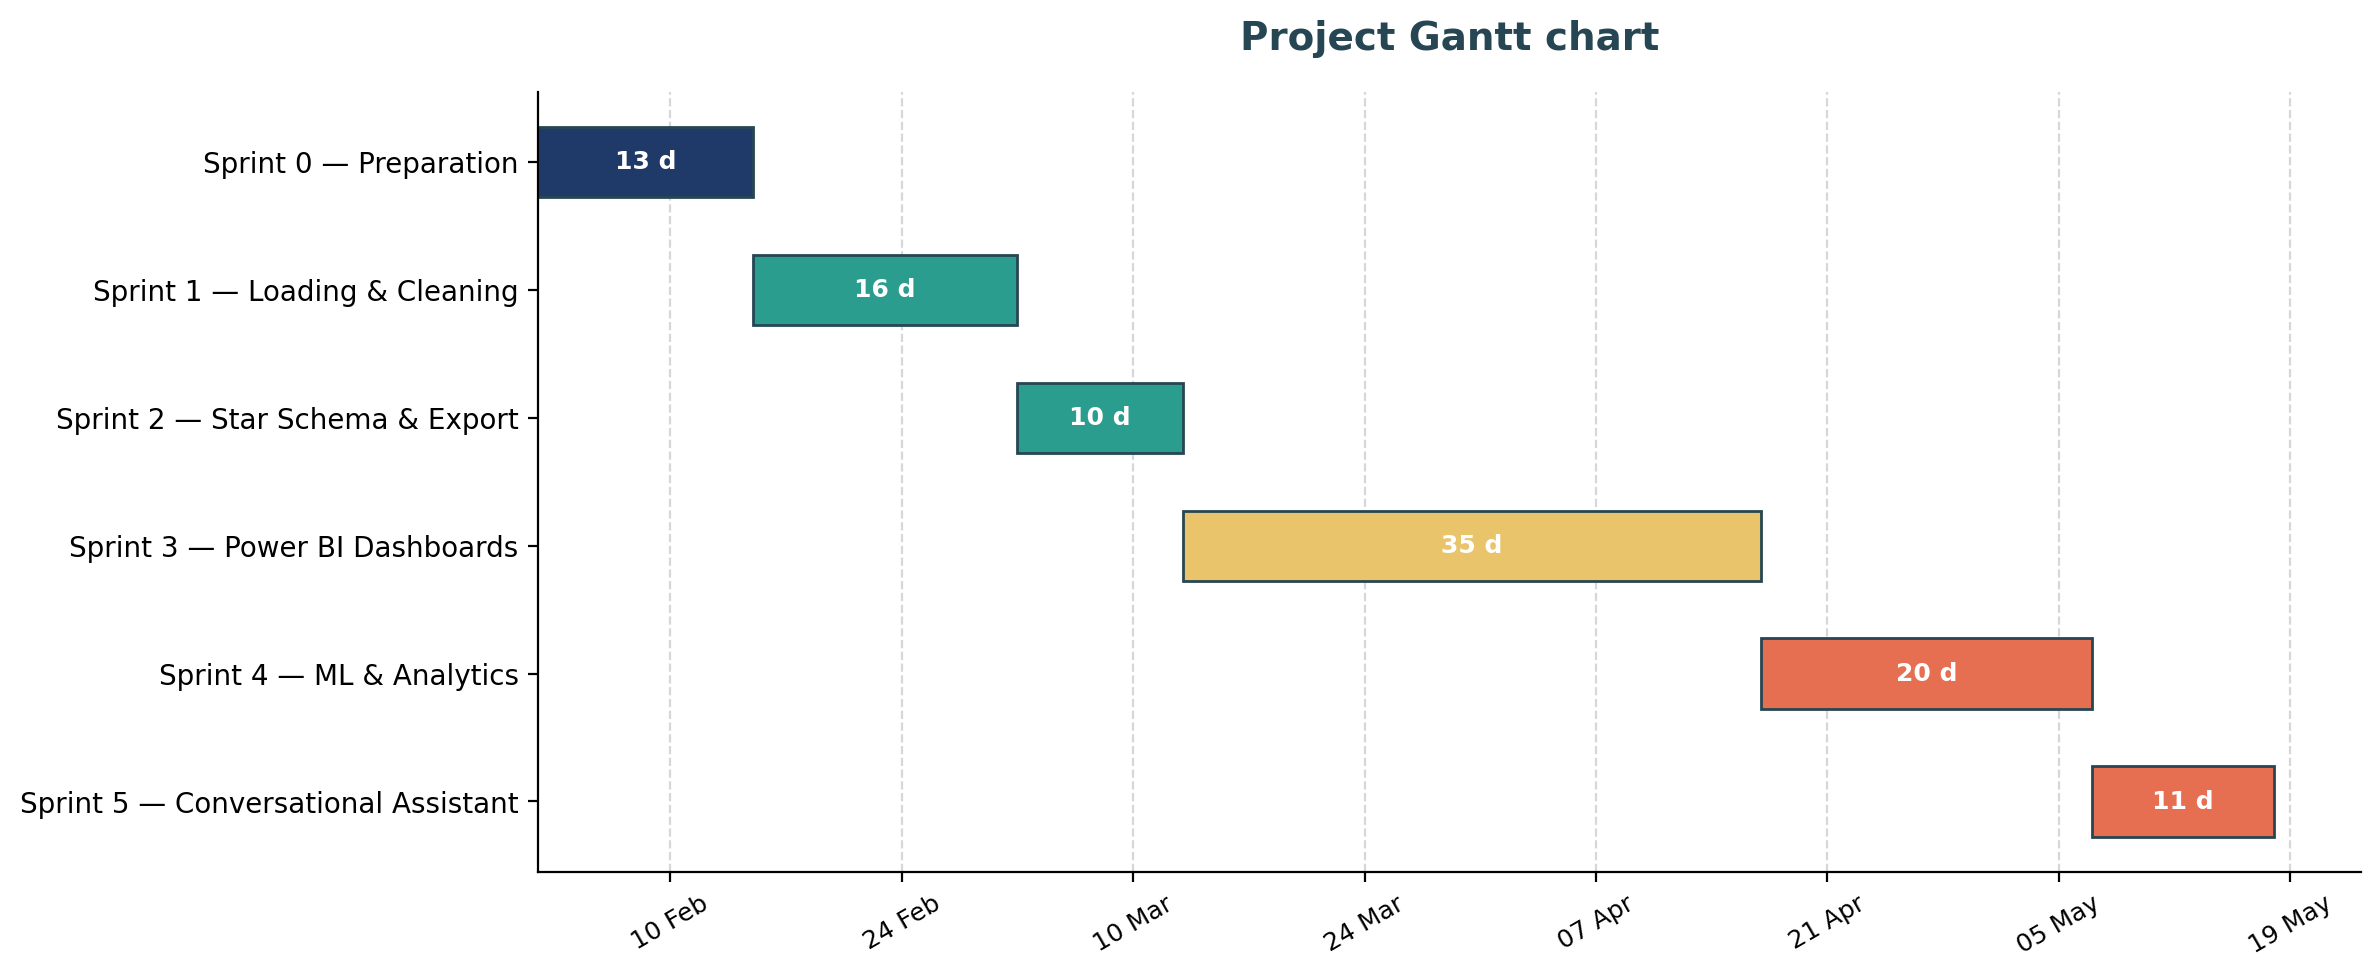
\includegraphics[width=\textwidth]{images/gantt.png}
  \caption{Project Gantt chart.}
  \label{fig:gantt}
\end{figure}

\section{Technical architecture of the decision-making solution}

The technical architecture of GamefyDB follows the classical ETL pattern
(Extract, Transform, Load), adapted to the specifics of the centre's data
and extended with an analytical layer and a conversational interface.
Figure~\ref{fig:architecture} walks through the successive layers
of the solution.

\begin{figure}[H]
  \centering
  
\includegraphics[width=0.95\textwidth]{images/pipeline.png}
  \caption{Technical architecture of the GamefyDB solution.}
  \label{fig:architecture}
\end{figure}

The architecture is organised in three layers.

\begin{itemize}
  \item \textbf{Data Collection:} the four source files exported by the
        point-of-sale software are stored in the \texttt{excel/} folder,
        together with a \texttt{weather\_tunis.parquet} cache for the
        Open-Meteo data and a set of synthetic \texttt{extended\_*.xlsx}
        files that supply the additional history required by the
        time-series models.
  \item \textbf{Data Integration:} a small set of focused Python modules
        carries the ETL chain and the analytical computations.
        \texttt{pipeline.py} cleans the raw files, fixes the typing, and
        builds the star schema. \texttt{forecaster.py},
        \texttt{segmenter.py}, and \texttt{anomaly\_detector.py}
        implement the machine-learning layer.
        \texttt{weather.py} provides the weather regressor. The whole
        layer is driven from a single entry point, namely
        \texttt{run.py}.
  \item \textbf{Data Delivery:} the output of the integration layer is
        written into two folders, \texttt{output/powerbi\_star/} for the
        star schema and \texttt{output/forecasts/} for the
        machine-learning outputs. Both folders are consumed directly by
        Power~BI and by the conversational assistant.
\end{itemize}

Before turning to the design of the warehouse itself in the next section,
three Business Intelligence notions on which the architecture rests deserve
a short definition: warehouses, subject-oriented marts derived from them,
and the integration chain that feeds both.

\begin{itemize}
  \item \textbf{Data Warehouse:} a centralised repository that
        consolidates information from several sources. Its tuning is
        oriented towards analytical workloads rather than transactional
        ones, and it gives fast access to both current and historical
        records so that strategic, cross-domain analyses become
        possible.
  \item \textbf{Data Mart:} a smaller, subject-focused slice of the
        warehouse, scoped to the analytical needs of a specific
        business unit or department. By exposing exactly the dimensions
        and measures that one audience cares about, a mart shortens the
        time it takes them to reach an answer.
  \item \textbf{ETL (Extract, Transform, Load):} the process in charge
        of pulling raw data out of the source systems, reshaping it so
        that it becomes consistent, complete and analytically usable,
        and writing the cleaned result into the target warehouse or
        mart.
\end{itemize}

\section{Overall design of the data warehouse}

The warehouse design is what the analytical layer ultimately rests
on. It dictates how the records are organised, stored and made
available to the rest of the solution, and a sensible layout is what
guarantees consistency, integrity and acceptable query latency for
both the dashboards and the machine-learning modules sitting above
it.

\subsection{Data Collection}

Data collection is a fundamental step of any Business Intelligence
initiative, since the quality of the collected data conditions the quality
of every subsequent analysis. For the present project, the data was
obtained from the centre's point-of-sale software in the form of four
\texttt{.xls} files exported on demand. Together, these files cover the
activity recorded between September~2025 and April~2026 and constitute the
only source of operational information available at the centre.
Table~\ref{tab:sourcefiles} describes the four files.

\begin{table}[H]
  \centering
  \caption{Source files and their contents.\label{tab:sourcefiles}}
  \begin{tabular}{p{4.2cm} p{8.3cm}}
    \toprule
    \textbf{File} & \textbf{Contents} \\
    \midrule
    \texttt{Cash DATA 01-09-2025.xls}
      & One row per cash transaction. Columns include the cashier, the
        datetime, the income or expense type, the payment method, the
        category, and the amount in TND. \\[4pt]
    \texttt{DATA session reports 01-09-2025.xls}
      & One row per gaming session. Columns include the cashier, the
        terminal, the session type, the duration, and the revenue split
        between usage, orders, USB data, and discount. \\[4pt]
    \texttt{Stock DATA 01-09-2025.xls}
      & One row per stock movement. Columns include the cashier, the
        datetime, the item name, the category, the movement direction
        (in or out), the quantity, the unit price, and the total. \\[4pt]
    \texttt{memeber DATA 01-09-2025.xls}
      & One row per loyalty member, containing cumulative statistics:
        total session duration, usage spend, order spend, USB spend, and
        overall total spend. The misspelled token \textit{memeber} is
        part of the actual filename and is preserved as such. \\
    \bottomrule
  \end{tabular}
\end{table}

\subsection{Key Performance Indicators (KPIs) Selection}

The Key Performance Indicators are the measures that the dashboards and
the forecasts will track on behalf of the manager. Their selection took
place during Sprint~0 in close collaboration with the Product Owner. The
KPIs were grouped into five thematic modules, namely revenue, sessions,
stock, members, and forward-looking analytics, as summarised in
Table~\ref{tab:kpis}.

\begin{table}[H]
  \centering
  \caption{KPI groups and their associated measures.\label{tab:kpis}}
  \begin{tabular}{p{3cm} p{10cm}}
    \toprule
    \textbf{Group} & \textbf{KPIs} \\
    \midrule
    Revenue
      & Total income (TND), total expenses (TND), net income, revenue
        split by payment method, revenue split by cashier, revenue split
        by transaction category, month-over-month revenue change,
        average transaction value. \\[4pt]
    Sessions
      & Total number of sessions, average session duration (in minutes),
        free-versus-paid split, total discount granted, session revenue
        per terminal and per terminal type. \\[4pt]
    Stock
      & Total units sold per item, total snack-bar revenue, average unit
        price per item, current stock level. \\[4pt]
    Members
      & Number of active members, average spend per member, total
        session duration across all members, orders transferred between
        members, USB-data usage, and distribution of the loyalty score. \\[4pt]
    Forward-looking
      & Revenue forecast over four weeks and three months with
        confidence intervals, member-activity forecast, peak-hour and
        peak-day profile, per-item restocking recommendation, and
        anomaly-flagged dates classified by series and by severity. \\
    \bottomrule
  \end{tabular}
\end{table}

\subsection{Data Warehouse Design Approaches}

Warehouse design is one of the make-or-break steps of any Business
Intelligence solution. A warehouse holds historical, consolidated
records, all aligned on the subjects the business cares about, so
that reporting and analytical queries can be answered efficiently.
Two reference methodologies tackle the design problem from opposite
ends: the Inmon approach and the Kimball approach. They differ in their philosophy
and in the way they organise the data, and the choice between them has
direct consequences on the analytical layer that sits above the warehouse.

\subsubsection{Inmon Approach}

The Inmon approach, developed by Bill Inmon, is also called the
\textit{top-down} approach. It recommends starting with the construction of
a centralised and fully normalised enterprise data warehouse that covers
the entire organisation. Subject-oriented data marts are then derived from
the central warehouse as analytical needs arise. The normalisation step
keeps the redundancy low and provides a single source of truth across the
organisation. The main drawback of this approach is the long delay between
the start of the project and the delivery of the first usable report,
since the entire warehouse must be designed before any analysis can take
place.

\subsubsection{Kimball Approach}

The Kimball approach, defended by Ralph Kimball, follows the opposite
direction and is often described as \textit{bottom-up}. Each business
process is captured as a self-contained star, and integration between the
different stars is achieved later through shared, conformed dimensions.
The core technique is dimensional modelling: numerical measures live in
fact tables, descriptive attributes live in dimension tables, and the two
families are wired together in a star (or, when normalisation is pushed
further, a snowflake) layout. The trade-off is well known: analysts get
something usable quickly, but a degree of redundancy across the various
marts has to be accepted.

\subsubsection{Adopted Approach}

Kimball is what was retained here. The context of the internship
backs that choice. The number of business domains involved is
small (four), the establishment operates on a single physical site, and
the timeline of the internship leaves no room for the prior design of a
full enterprise data warehouse. With Kimball, each output table could be
validated against the real data during Sprint~2 and adjusted whenever
needed before the work moved on to the next table. The conformed
dimensions \textit{dim\_cashier} and \textit{dim\_terminal} provide the
cross-domain integration that the Kimball methodology requires, while the
overall model remains compact and easy to maintain.

\section{Multidimensional Modeling}

Multidimensional modelling is a fundamental concept of Business
Intelligence and data warehousing. The records are split between
fact tables (the measurable events) and dimension tables (the
descriptive context) so that analytical queries read naturally and
run efficiently. A fact table contains the quantitative measures that
describe the business events being analysed. The dimension tables, in
turn, contain the descriptive attributes that allow the user to slice the
facts along multiple analytical axes such as time, location, product, or
customer.

\subsection{Conceptual Model Analysis}

The design of the conceptual model is the step in which the data is given
its analytical structure prior to any physical implementation. Three
dimensional patterns are commonly used in Business Intelligence, and they
were all considered as candidates for the conceptual model of GamefyDB.

\begin{itemize}
  \item \textbf{Star Schema Model:} the star schema is composed of a
        single central fact table surrounded by dimension tables. Its
        simplicity makes it well suited to analytical queries and
        supports fast data retrieval in data-warehousing environments.
  \item \textbf{Snowflake Schema Model:} the snowflake variant pushes
        normalisation one step further by splitting each dimension into
        a small chain of related sub-dimensions. Redundancy is reduced
        but queries pay the price in extra joins at execution time.
  \item \textbf{Galaxy Schema Model (Fact Constellation):} the galaxy
        schema involves several fact tables that share a set of common
        dimension tables. It enables the simultaneous analysis of
        multiple business processes from a consistent set of dimensions.
\end{itemize}

\subsection{Choice of the Conceptual Model}

For the GamefyDB project, a \textbf{galaxy schema} (fact constellation)
was retained. The choice is motivated by the structure of the data
itself. Two fact tables, \textit{fact\_transaction} and
\textit{fact\_session}, share three conformed dimensions
(\textit{dim\_cashier}, \textit{dim\_terminal}, and \textit{dim\_member}),
while a fourth dimension, \textit{dim\_item}, is referenced only by
\textit{fact\_transaction} since the items appear exclusively in the
context of order-income transactions. The stock movements and the
cumulative per-member statistics were absorbed directly into
\textit{dim\_item} and \textit{dim\_member} respectively, during the
design refinement carried out in Sprint~2. There is only one direction of
stock movement in practice (out-of-stock sales), and the members file is
cumulative rather than event-based, which makes a dedicated fact table
unnecessary in both cases. Figure~\ref{fig:starschema} represents the
resulting conceptual model, and Table~\ref{tab:star_schema} lists the six
output tables and the key columns that they expose.

\begin{figure}[H]
  \centering
  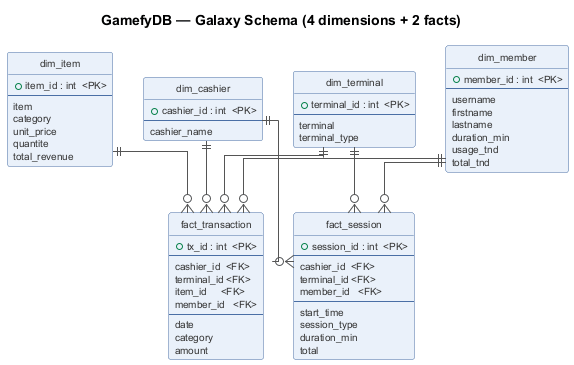
\includegraphics[width=\textwidth]{images/star_schema.png}
  \caption{Conceptual model of the GamefyDB data warehouse.}
  \label{fig:starschema}
\end{figure}

\begin{table}[H]
  \centering
  \caption{Output tables of the GamefyDB star schema.\label{tab:star_schema}}
  \begin{tabular}{lll}
    \toprule
    \textbf{Type} & \textbf{Table} & \textbf{Key columns} \\
    \midrule
    Dimension & \texttt{dim\_cashier}  & cashier\_id (PK), cashier\_name \\
    Dimension & \texttt{dim\_terminal} & terminal\_id (PK), terminal, terminal\_type \\
    Dimension & \texttt{dim\_item}     & item\_id (PK), item, category, unit\_price, \\
              &                        & quantite, total\_revenue \\
    Dimension & \texttt{dim\_member}   & member\_id (PK), username, firstname, lastname, \\
              &                        & duration\_min, usage\_tnd, orders\_tnd, total\_tnd \\
    \midrule
    Fact & \texttt{fact\_transaction} & tx\_id (PK), cashier\_id (FK),
                                        terminal\_id (FK, nullable), \\
         &                            & item\_id (FK, nullable),
                                        member\_id (FK, nullable), \\
         &                            & date, category, amount \\
    Fact & \texttt{fact\_session}     & session\_id (PK), cashier\_id (FK),
                                        terminal\_id (FK), \\
         &                            & member\_id (FK, nullable),
                                        session\_type, duration\_min, \\
         &                            & order\_transfer, usage, discount, total \\
    \bottomrule
  \end{tabular}
\end{table}

\section{Work Environment}

This section presents the hardware and the software environment in which
the work was carried out. The hardware constraints had no major influence
on the design of the solution, since all the computations involved fit
comfortably on a single workstation. The software stack, by contrast, was
chosen carefully, since each component is used at one or several stages of
the pipeline.

\subsection{Hardware environment}

The work was conducted on a personal laptop whose specifications are the
following:

\begin{itemize}[noitemsep]
  \item \textbf{Type:} laptop.
  \item \textbf{Brand:} Lenovo, model 83DV.
  \item \textbf{Processor:} Intel Core i7-13650HX (13th generation),
        14 cores and 20 threads.
  \item \textbf{Memory:} 32~GB of RAM.
  \item \textbf{Storage:} 500~GB MSI M450 SSD and 512~GB Micron NVMe SSD.
  \item \textbf{Graphics:} NVIDIA GeForce RTX 4050 Laptop.
  \item \textbf{Operating system:} Windows~11 Pro.
\end{itemize}

\subsection{Software environment}

Most of the work runs in Python; the rest is whatever was needed to
read the source files, query an API or render a report. The stack is
described below, grouped by what each piece actually does in the
project rather than alphabetically.

\paragraph{Python.} Every script, module and notebook in this project
is written in Python (version 3.14). The pipeline, the
machine-learning modules, the data generator, the helper scripts and
the chatbot all live in the same monorepo and share the same
interpreter --- which keeps the dependency story short and the
debugging loop fast.

\paragraph{xlrd, openpyxl, pandas, NumPy.} Tabular work goes through
pandas and NumPy. The ingestion stage is the only place where xlrd
appears, and only because the members file refuses to open through
\texttt{pandas.read\_excel} (more on that in Chapter~3). For the
extended \texttt{.xlsx} files written by the synthetic generator, the
pipeline switches to openpyxl, which handles the newer format
cleanly.

\paragraph{Forecasting stack: Prophet, pmdarima, XGBoost.}
Three algorithms were put head to head in Sprint~4 so the choice of a
production model is justified rather than asserted. Prophet
(Meta's additive decomposition) carries the production forecast and
also accepts the Tunis weather as an external regressor. pmdarima
wraps SARIMA behind a single \texttt{auto\_arima} call so the
seasonal and non-seasonal orders are picked automatically. XGBoost
sits in the same evaluation harness with hand-engineered lag and
calendar features.

\paragraph{scikit-learn and statsmodels.} K-Means comes from
scikit-learn (along with its \texttt{StandardScaler}, which matters
more than it sounds --- without it the spending feature would dominate
the cluster distances). statsmodels supplies the Augmented
Dickey-Fuller test that anchors the stationarity diagnostic.

\paragraph{matplotlib.} Every PNG in the report's analytics chapters
--- accuracy plots, segmentation scatters, peak-hour bars, anomaly
timelines, the model-comparison chart --- is rendered with
matplotlib. The figures live under \texttt{docs/} and regenerate as
part of \texttt{python run.py}.

\paragraph{requests.} The Open-Meteo client in
\texttt{gamefydb/weather.py} is built on top of requests. Responses
are cached to \texttt{excel/weather\_tunis.parquet} so repeated
pipeline runs hit the network exactly once.

\paragraph{Streamlit.} The chatbot front-end is a Streamlit app
(\texttt{app.py}). The framework was picked over Flask or FastAPI
mainly because it gave the multilingual layout, the voice-input
component slot and the conversation state for free.

\paragraph{Microsoft Power~BI.} All four dashboard pages of
\texttt{gamefyyy.pbix} live inside Power~BI Desktop, which loads the
six CSV files of the star schema and the analytics outputs, holds
the data-model relationships, and stores the DAX measures.

\paragraph{Auxiliary tools.} pytest runs the test suite that
backs the parsing, cleaning, segmentation, anomaly-detection and
weather modules. PlantUML renders the use-case, pipeline and
star-schema diagrams from \texttt{.puml} sources committed alongside
the report. Visual Studio Code is the editor (with the Python and
PlantUML extensions), Git and GitHub track and host the source code,
and Overleaf is where this \LaTeX{} report is written and compiled.

\section{Conclusion}

By the end of Sprint~0 there is still no code shipping, but most of the
risk has been retired: the actors are known, the backlog has been
ordered with the Product Owner, the schedule has six labelled sprints
in it, the three-layer architecture is drawn, and the galaxy schema
has been sized down from eight tables to six after a closer look at
what the source files actually contain. The work environment is
documented too, so a second machine can be set up later without
guesswork. Sprint~1 takes over from here and begins the implementation
proper, starting where every BI project of this kind sooner or later
has to start --- at the raw \texttt{.xls} files.

% ============================================================
\end{document}
